\chapter{Light Field Microscope}
\label{chap:microscope}
\markboth{\MakeUppercase{Light Field Microscope}}{}
The laboratory setup of a light field microscope was developed to verify the results obtained in the simulations and to extend the knowledge of plenoptic imaging systems from theory to practice. This prototype is a versatile and flexible instrument built with the purpose to test and explore all the potential of light field imaging for microscopy applications. The philosophy was to realize a setup with the maximum number of degrees of freedom possible in order to test a wide variety of configurations of the optical parameters as done previously in the simulation platform.\\
 In the next sections the design parameters and guidelines used to develop the setup will be presented. A protocol to acquire and render images will be described and examples of rendered images acquired with the experimental setup will be shown. 
\section{From Simulation to Reality}
The results obtained in the simulation have been used as a guideline for the process of developing a working system. It has been clear since the beginning that a 1.0 system would not be the best option for a laboratory setup as:
\begin{itemize}
	\item a plenoptic 1.0 imaging system, as explained in section \ref{sec:camera10}, requires the lenslet array to be conjugated to the object plane, and the sensor plane to be conjugated with the main lens. To satisfy this condition along with the f-number matching, the micro array should be placed at a distance to the sensor equal to its focal length with great precision \cite{ng2006digital,ng2005light,levoy1996light,levoy2006microscope}. To achieve this degree of precision advanced machinery and a clean room is needed in order to fabricate a custom lenslet array. Ideally its focal length should be equal to the lenslets substrate thickness and then stuck it to the sensor. A solution to bypass this issue is to build a relay system of lenses between the micro lens array and the sensor, as done by Adelson and Wang in 1992, \cite{adelson1992single} adding complexity and cost to the system.
	\item the spatial resolution is limited by the number of lenslets in the array. The ideal condition to achieve high resolution images is to have an array with a small pitch and a large number of lenslets. The sensor should also be large with small pixel size, increasing the costs. For example to achieve a resolution of 1000 by 1000 pixels in the final rendered image, if the lenslets have an aperture diameter of 150 $\mu m$ as the one used in section \ref{sec:system10}, the array should be 15 by 15 cm wide and the sensor should have a resolution of 30000 by 30000 pixels.
\end{itemize}
Hence from a practical point of view building a proper plenoptic 1.0 system can be expensive and complicated considering the performance achieved in terms of resolution. \\
A plenoptic 2.0 on the other hand it is easier to build and gives better results in terms of spatial and directional resolution trade off. The key variable to control is the distance between the micro lens array and the sensor. In order to replicate some of the simulations done, a system with a tunable micro array position was designed and developed as explained in detail in the next sections.
\section{Description of the System}
The system has been designed following the guidelines given by Georgiev and Intwala \cite{georgiev2006light}. The assembly of the system uses Linos microbench system and components (Qioptip, USA).
With reference to figure \ref{fig:realsys}, a system working in transmission was built. It is composed of four main parts: 
\begin{itemize}
	\item Illumination: composed of an LED array lamp, a diffuser and a condensing lens are used to concentrate the maximum area of the light source on the sample. A K\"ohler illumination lens has been added in order to generate an even illumination on the sample removing artefacts generated by imaging the light source on the object \cite{kohler1893new,kohler1934device}. 
	\item The main optics: its role is to form an image of the object in front of the micro lens array. It consists of a 2f system, with a single lens as described in chapter \ref{chap:chapter1}.
	\item Micro lens array: The micro lens array is a relay system between the main lens image and the sensor of the microscope. It defines the trade-off between optical and spatio-angular resolution.
	\item Sensor plane: it records the light field. It should be large enough to capture all the light coming from the lenslet array and it should provide enough resolution to have high resolution sub images.
\end{itemize}
Figure \ref{fig:realsys} shows a schematic diagram of the setup. The illumination system was made by an LED light source (Thorlabs Inc. LED array LIU630), with a central wavelength of 630 nm, an output power of 208 mW and an emission spectrum shown in figure \ref{fig:emission_spectrum} with a full width half maximum of 20 nm as already discussed in \ref{sec:simtempcoherence}.
\\
A condensing lens with a focal length of 27 mm has been placed in front of the light source to maximise the light reaching the sample reducing the divergence of the LED array light source. The image formed by the condensing lens has been relayed by the K$\ddot{o}$hler lens on the main lens of the system. In this way the structure of the light source is not affecting the quality of the image \cite{kohler1893new}. To make it even more uniform a diffuser has been placed between the LED source and the condensing lens, as shown in figure \ref{fig:realsys}.\\
The main optics consisted of two plano-convex lenses with a focal length of 120 mm each placed one next to the other as shown in figure \ref{fig:realsys} so that they form a main lens with a total focal length of 60 mm. The two lenses have been mounted with the flat surface facing outwards to minimize spherical aberrations. The main lens was in a 2f configuration, producing an image with a magnification of -1 on the main lens image plane. 
\newpage
\begin{figure}[H]
	\centering
	\includegraphics[width=.9\textwidth]{C:/Users/Massimo/Documents/Thesis/Thesis_PhD/realsystem.eps}
	\caption{\label{fig:realsys} Schematic diagram of the light field microscope. The values of the distances are: $z_c$=27 mm, $z_k$=120 mm, $z_1$=$z_2$=120 mm.
 }
\end{figure}
The plenoptic stage is the most complex part of the system. Its optical properties are defined by the magnification of the micro array stage \cite{turola2014wave,georgiev2010focused}, therefore in an optical setup this parameter should be tuned with high accuracy in order to produce a rendered image with the desired resolution. The correct tuning of the magnification is achieved by defining the appropriate values for the lengths \textit{a} and \textit{b}. Because of the parabolic nature of the lens law small variations in one of the parameters could produce undesired effects on the image.\\
The technical solution adopted was to use two micrometric mechanical translation stages to move with precision both the whole plenoptic stage with respect to the main lens and the sensor as illustrated in figure \ref{fig:traslator}. The first translator moves the whole plenoptic stage, made of the sensor and microarray, with respect to the main lens tuning the distance between the main lens image and the micro lens array (\textit{a}). Once \textit{a} is set the second translator moves the sensor with respect to the microlens array, setting the distance between the microarray and the sensor \textit{b}. For each pair \textit{(a, b)}, only one value of the micro array magnification is defined. A further degree of freedom is represented by the possibility to move the micro array perpendicularly to the optical axis in \textit{x} and \textit{y} in order to centre the array with the sensor.
Figure \ref{fig:photo} shows the assembled light field recording stage and the locations of the two micro metric translators are indicated.
\begin{figure}[H]
	\centering
	\includegraphics[width=.9\textwidth]{C:/Users/Massimo/Documents/Thesis/Thesis_PhD/traslator.eps}
	\caption{\label{fig:traslator} Schematics of the light field recording stage. The first micro metric translator moves both the sensor and micro array stages. The second only moves the micro array stage with respect to the sensor stage. }
\end{figure}
\begin{figure}[H]
	\centering
	\includegraphics[width=.7\textwidth]{C:/Users/Massimo/Documents/Thesis/Thesis_PhD/photosys.eps}
	\caption{\label{fig:photo} Assembled light field recording stage with. }
\end{figure}
The micro array used (MLA150-5c-M, Thorlabs Inc, USA) has a 10 mm $\times$ 10 mm square grid made of 146 $\mu$m diameter plano-convex lenslets on a substrate of fused silica. The lenslet pitch is 150 $\mu$m. All the geometric parameters of the lenslet array can be seen in figure \ref{fig:micro array} where \textit{r} is the radius of curvature of the lenslet, \textit{s} is the height of the lenslet from the substrate, \textit{p} is the pitch, \textit{t} the thickness of the substrate and \textit{f} is the focal length. It is linked to the radius of curvature by the relation:
\begin{equation}
	\label{eq:f_micro}
		f = \dfrac{r}{n-1}
\end{equation} 
where \textit{n} is the refractive index of the lenslet array.
Assuming the diameter of each lenslet almost equal to the pitch, the radius of curvature is linked to the other geometrical parameters by the relation \cite{herzig1997micro}: 
\begin{equation}
\label{eq:r_micro}
r = \dfrac{s^2+\frac{p^2}{4}}{2s}
\end{equation} 

\begin{figure}[H]
	\centering
	\includegraphics[width=.6\textwidth]{C:/Users/Massimo/Documents/Thesis/Thesis_PhD/microarray2.eps}
	\caption{\label{fig:micro array} Lenslet array parameters.}
\end{figure}
 The raw image is recorded using a 10 megapixel CMOS technology sensor with 3840 by 2748 pixels extracted from a digital camera (UI-1490LE-C-HQ, IDS Imaging Development System GmbH, Germany). Its pixel size is 1.67 $\mu$m with a sensor size of 6.413 mm $\times$ 4.589 mm mounted at on the back of the translation stage. \\
 In order to control the position of the micro array the two translators should be shifted by a quantity \textit{c} and \textit{d}. \textit{c} is the shift of the first translator and set the parameter \textit{a} while \textit{d} is the shift to apply to the second translator, setting \textit{b}. The values of \textit{c} and \textit{d} are listed in table \ref{tab:7}.
 For each pair \textit{(c, d)}, table \ref{tab:7} shows for the corresponding optical parameters: the f-number $F_\#$, the numerical aperture \textit{NA} the cut-off frequencies of the main lens and of the plenoptic stage $\nu$. This parameters define the theoretical optical performances of the prototype and have been calculated with the same method used in section \ref{sec:performances}.
 \newpage
\begin{sidewaystable}[]
	\centering
	\label{tab:7}
	\scalebox{0.8}{
	\begin{tabular}{lllllllll}
		Magnification & a (m)     & b (m)   & NA          & F\#         & $\nu$ Main lens (cycle/m) & $\nu$ Plenoptic (cycle/m) & $c$ (m)   & $d$ (m)       \\
		0             & 0           & 0.0052  & 0.01442 & 34.6667 & 22785.2716            & 0                     & 0.0052  & 0.0000           \\
		0.1           & 0.05720      & 0.00572 & 0.01311 & 38.1334 & 20713.8832           & 2071.3883           & 0.0057 & 0.0515     \\
		0.15          & 0.03987 & 0.0060 & 0.0125 & 39.8667 & 19813.2797           & 2971.9919           & 0.0060 & 0.0339 \\
		0.2000           & 0.0312      & 0.0062 & 0.0120 & 41.6000        & 18987.7263           & 3797.5452           & 0.0062 & 0.0250     \\
		0.2500          & 0.0260       & 0.0065  & 0.0116 & 43.3334 & 18228.2173           & 4557.0543            & 0.0065  & 0.0195      \\
		0.3           & 0.02253 & 0.0068 & 0.0111 & 45.0667 & 17527.1320             & 5258.1396             & 0.0068 & 0.0158 \\
		0.35          & 0.0201 & 0.0070 & 0.0107 & 46.8000        & 16877.9790           & 5907.2926           & 0.0070 & 0.0130 \\
		0.4000           & 0.0182      & 0.0073 & 0.0103 & 48.5334 & 16275.1940             & 6510.0776             & 0.0073 & 0.0109     \\
		0.45          & 0.0168 & 0.0075 & 0.0099  & 50.2667 & 15713.9804           & 7071.2912           & 0.0075 & 0.00922 \\
		0.5           & 0.0156      & 0.0078  & 0.0096 & 52.0000          & 15190.1811           & 7595.0905           & 0.0078  & 0.0078      \\
		0.55          & 0.0147 & 0.0081 & 0.0093 & 53.7334 & 14700.1752           & 8085.0964           & 0.0081 & 0.0066 \\
		0.6           & 0.0139 & 0.0083 & 0.0090 & 55.4667 & 14240.7945           & 8544.4765            & 0.0083 & 0.00555 \\
		0.65          & 0.01320      & 0.0086 & 0.0087 & 57.2000        & 13809.2555           & 8976.0160           & 0.0086 & 0.0046     \\
		0.7           & 0.0126 & 0.0088 & 0.0085 & 58.9334 & 13403.1009           & 9382.1707           & 0.00884 & 0.0038 \\
		0.75          & 0.0121 & 0.0091  & 0.0082 & 60.6667 & 13020.1552            & 9765.1164             & 0.0091  & 0.0030 \\
		0.8           & 0.0117      & 0.0094 & 0.0080 & 62.4000        & 12658.4842           & 10126.7874           & 0.0094 & 0.0023     \\
		0.85          & 0.0113 & 0.0096 & 0.0078 & 64.1334 & 12316.3630           & 10468.9086           & 0.0096 & 0.0017 \\
		0.9           & 0.0110 & 0.0098 & 0.0076 & 65.8666 & 11992.2482           & 10793.0234           & 0.0099 & 0.0011 \\
		0.95          & 0.0108 & 0.01014 & 0.0074  & 67.6000        & 11684.7547           & 11100.5169           & 0.0101 & 0.0005 \\
		1             & 0.0104      & 0.0104  & 0.0072 & 69.3334 & 11392.6358            & 11392.6358            & 0.0104  & 0.0000          
	\end{tabular}
}
	\caption{Table containing the parameters of the micro lens array translation stage. \textit{a} and \textit{b} are the distances shown in figure \ref{fig:micro array}, while \textit{c} and \textit{d} are the shift to apply to each translator to set the correspondent magnification value. This table also shows the optical parameters corresponding to the different positions of the translator.  }
\end{sidewaystable}
\section{Image Acquisition Protocol}
\label{sec:protocol}
The development of a new imaging system required the definition of a protocol to correctly record and render the plenoptic raw image. The protocol can be summarised as follows:
\begin{itemize}
	\item according to the magnification desired the parameters \textit{a} and \textit{bs} are set by moving the two translation stages by the quantities \textit{c} and \textit{d} indicated in table \ref{tab:7};
	\item the object is removed in order to capture a calibration image using a uniform pattern of monochromatic light;
	\item the aperture of the main lens is changed in order to satisfy the f-number matching condition;
	\item if necessary the position in \textit{x,y} of the micro array is adjusted as explained in detail below; 
	\item the object is put back in place and the raw image is captured;
	\item the final image is rendered using the basic rendering algorithm explained in section \ref{sec:rendering}.
\end{itemize} 
The calibration image is required to verify the correct alignment of the lenslet array and that the f-number matching condition is respected. It is also used as a guide to create the sub-images grid to render the final image. According to the calibration image, the position in x and y of the micro lens array can be adjusted translating it in x and y, rotating it and if necessary tilting it. These degrees of freedom allow to fine tune the position of the lenslets with respect to the sensor. This operation is performed manually checking the correct alignment on the monitor connected to the camera sensor. Figure \ref{fig:calibrationimg3} shows the four main conditions of micro array misalignment.
\begin{figure}[H]
	\centering
	\includegraphics[width=.6\textwidth]{C:/Users/Massimo/Documents/Thesis/Thesis_PhD/alignedarray.eps}
	\caption{\label{fig:calibrationimg3} Common causes of bad alignment between the micro lens array and the sensor. }
\end{figure}
The same image is used to match the f-number of the main lens with the one of the lenslet array according to the configuration of \textit{a} and \textit{b} chosen. This is done manually by changing the aperture placed in front of the main lens until sub images touch each others. Figure \ref{fig:calibrationimg1} shows the case where the aperture of the main lens is too small, and the gap between the sub images is too large while figure \ref{fig:calibrationimg2} shows the calibration image obtained once the aperture of the main lens has been adjusted to match the f-number.
\\
After the f-number is matched, it is possible to proceed with the acquisition of the raw image of the sample. In this case a USAF resolution target has been used as an object. Figure \ref{fig:rawreal} shows the raw images obtained with magnifications equal to 0.5 and 0.4, while figure \ref{fig:rawreal2} shows the raw images obtained with a magnification of 0.3 and 0.25.
\begin{figure}[H]
	\centering
	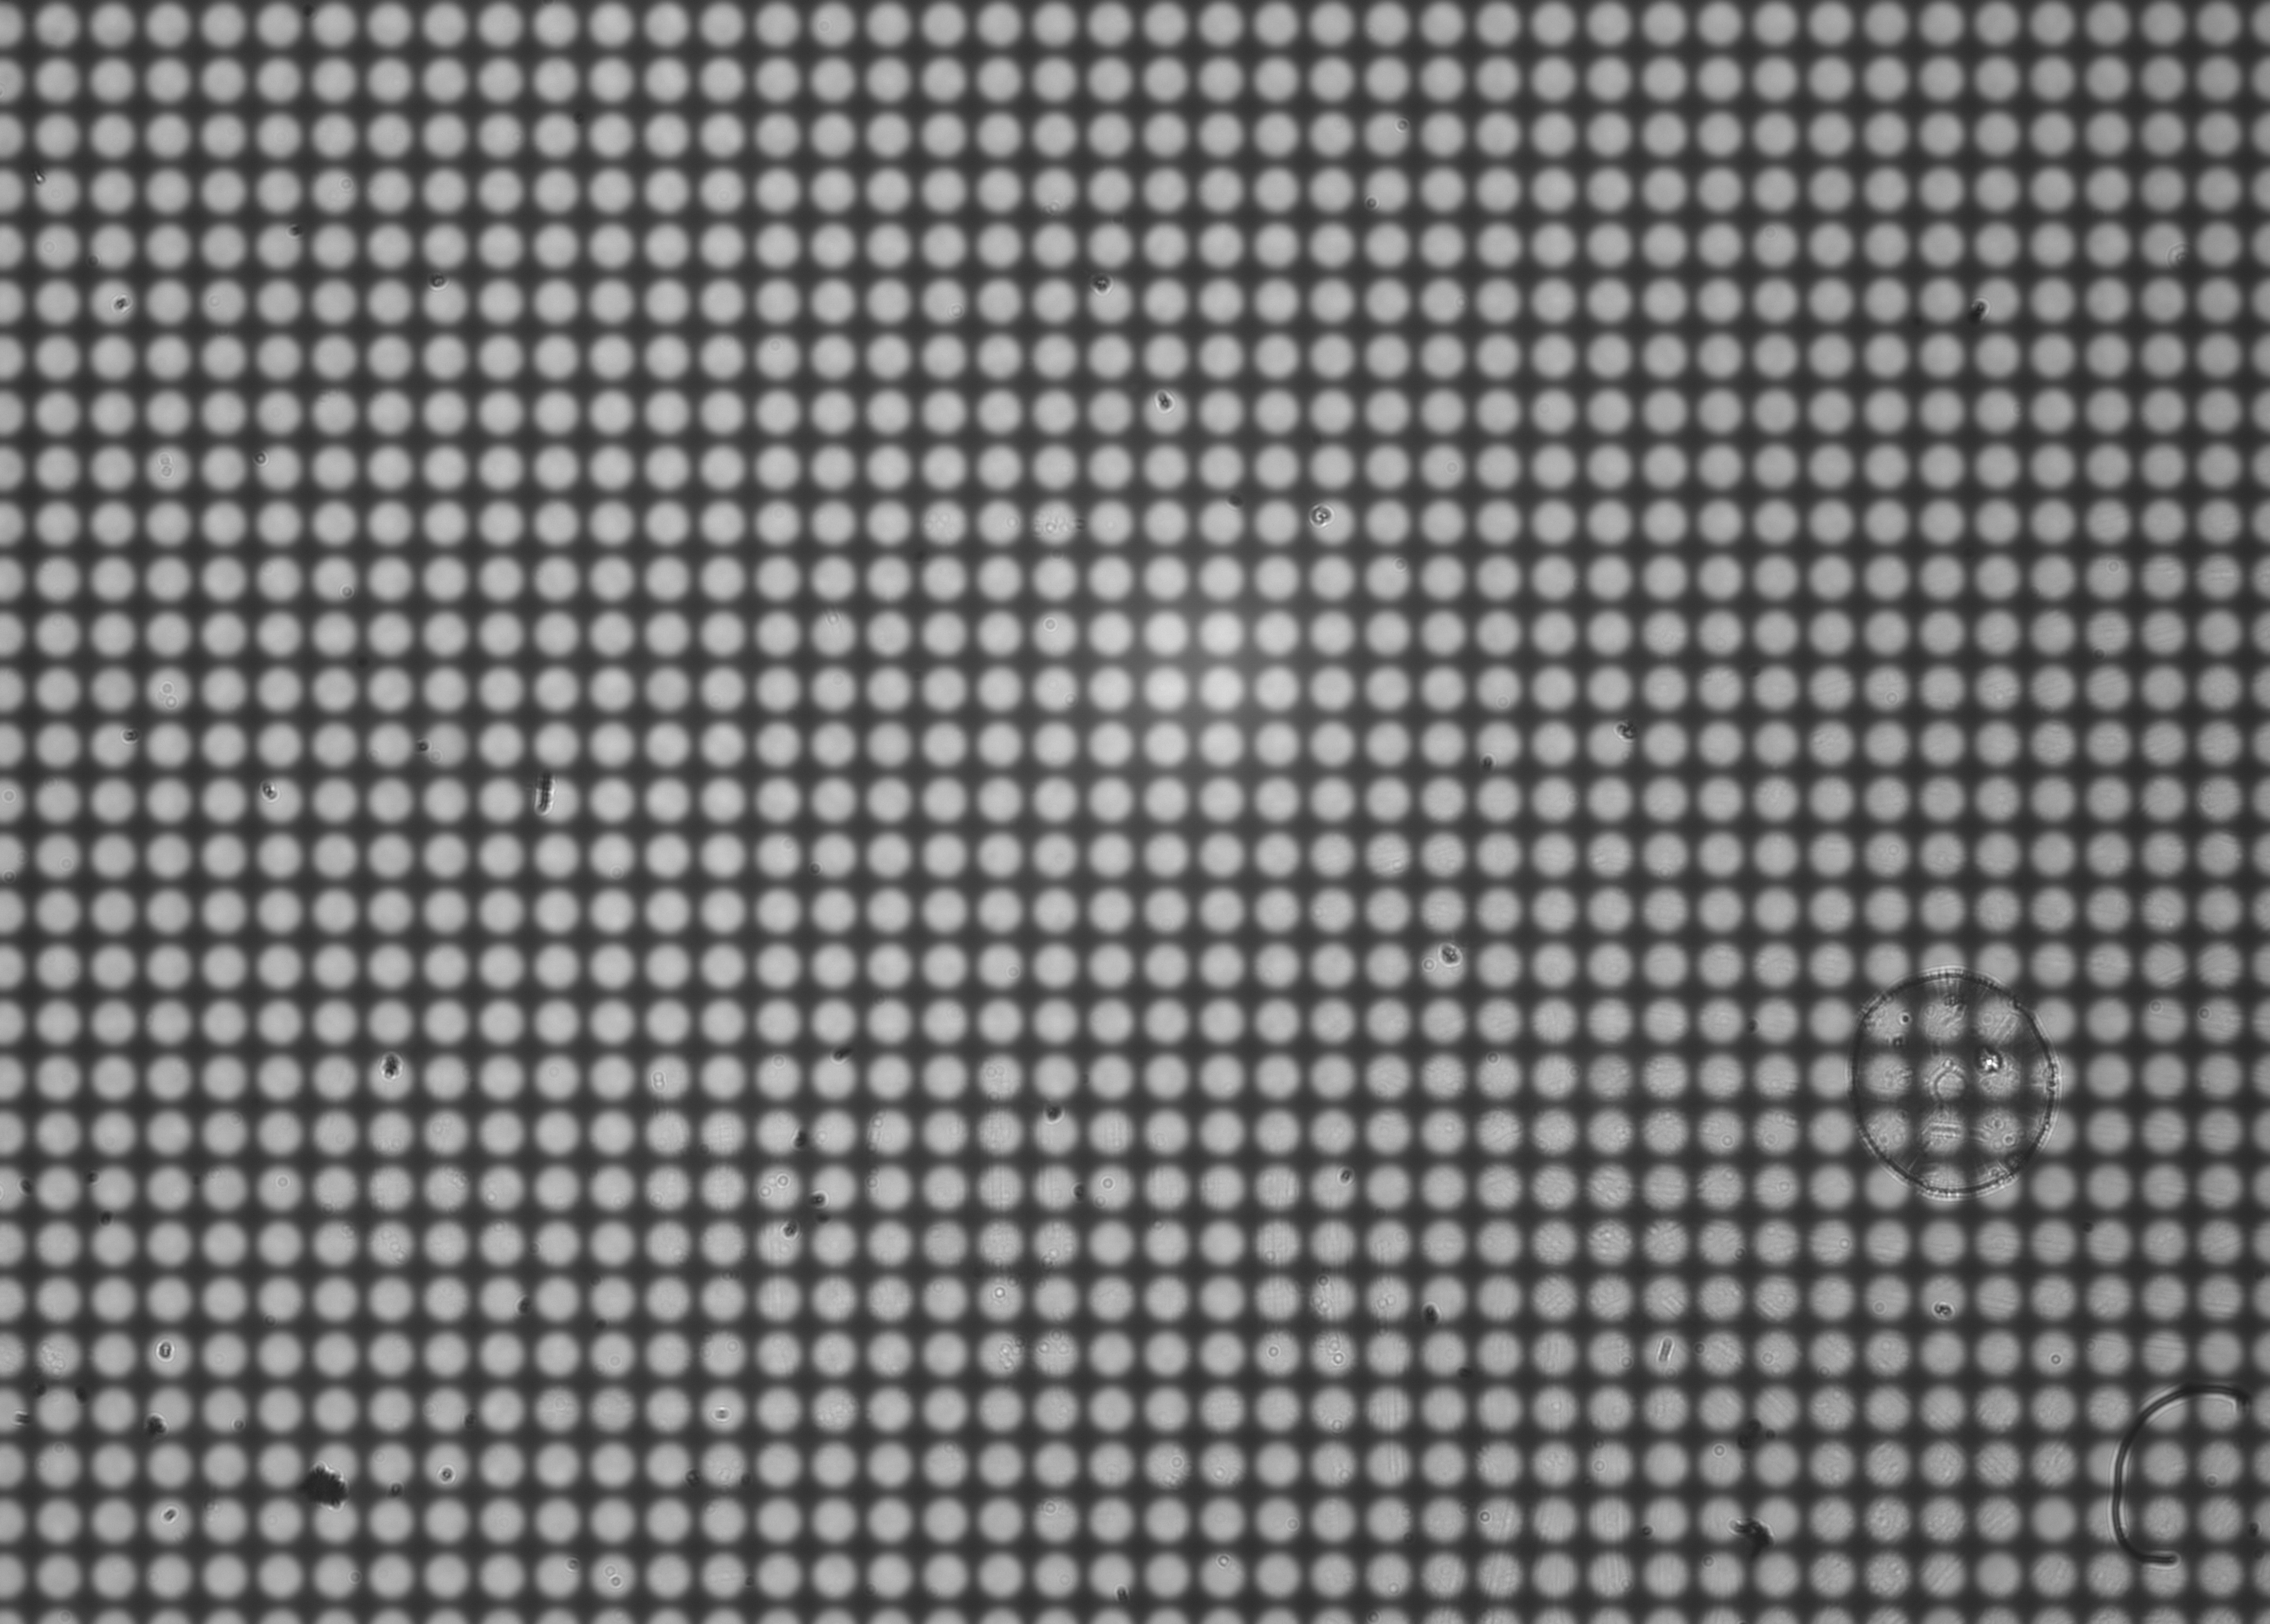
\includegraphics[width=.7\textwidth]{C:/Users/Massimo/Documents/Thesis/Thesis_PhD/homemade/PW05c.png}
	\caption{\label{fig:calibrationimg1} Calibration image with f-number not matched. }
\end{figure}
\begin{figure}[H]
	\centering
	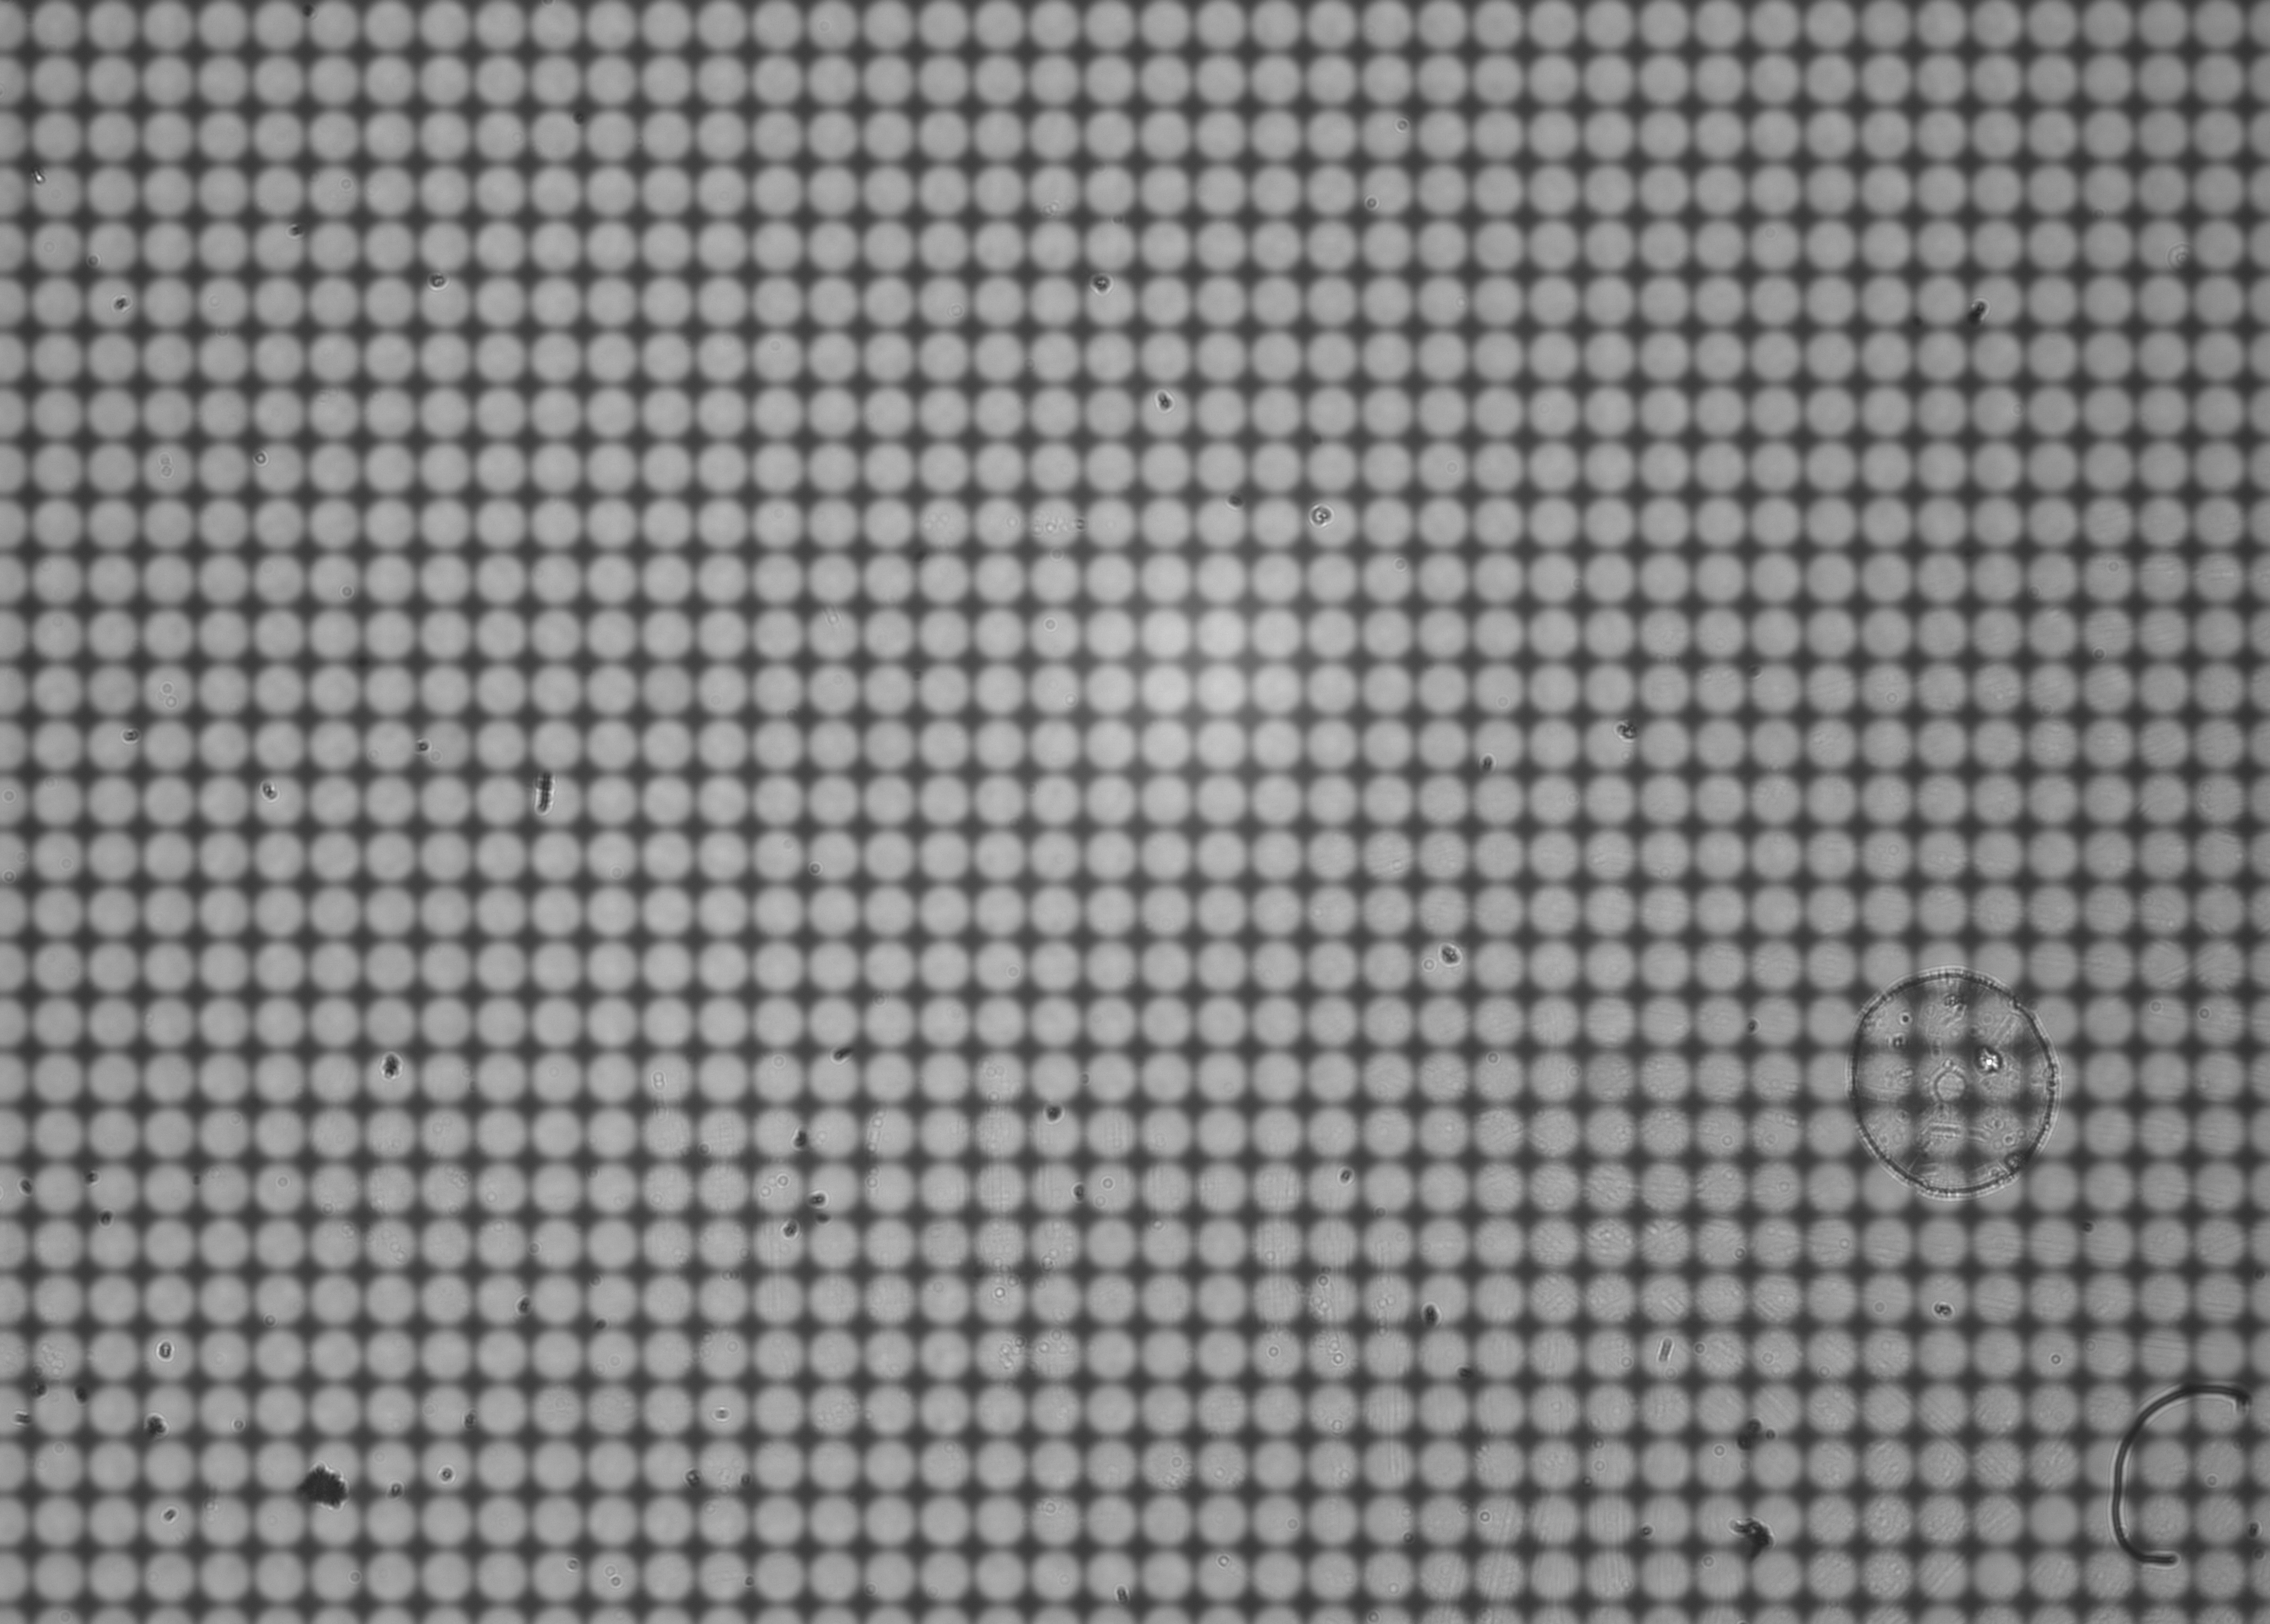
\includegraphics[width=.7\textwidth]{C:/Users/Massimo/Documents/Thesis/Thesis_PhD/homemade/PW05a.png}
	\caption{\label{fig:calibrationimg2} Calibration image with matched f-number. }
\end{figure}
\begin{figure}[H]
	\centering
	\includegraphics[width=.9\textwidth]{C:/Users/Massimo/Documents/Thesis/Thesis_PhD/raw0504.eps}
	\caption{\label{fig:rawreal} Raw plenoptic 2.0 image of the USAF resolution target obtained by the prototype system built in lab. The top image has a magnification of 0.5, the bottom 0.4. }
\end{figure}
\begin{figure}[H]
	\centering
	\includegraphics[width=.9\textwidth]{C:/Users/Massimo/Documents/Thesis/Thesis_PhD/raw03025.eps}
	\caption{\label{fig:rawreal2} Raw plenoptic 2.0 image of the USAF resolution target obtained by the prototype system built in lab. The top image has a magnification of 0.3, the bottom 0.25. }
\end{figure}
These raw images show how the different features of the target object are decomposed into sub images. The number of times each point of the main lens image is replicated under the lenslet array increases with decreasing magnification as explained in chapter \ref{chap:chapter1} and then verified from the simulations in chapter \ref{chap:chapter4}.
\newpage 
\section{Rendering of experimental data}
Rendering images from raw data acquired by the prototype of the light field microscope is more complicated then the case of the simulated raw data. While in a simulation the lenslet array is perfectly aligned with the other optical components, in a real system this is not true any more. Small tilts and non-alignments between the micro lens array and the sensor can produce inhomogeneity of the magnification along the grid. As a consequence the sub images size will vary along the grid. Although these differences are extremely small, usually around 10-15 pixels, they causes a distortion along the grid that is not predictable or quantifiable. For this reason it cannot be easily corrected, like in the case of the computer generated raw data in section \ref{sec:isolating} and artefacts will be produced during the rendering process. To avoid this a method to extract the information on the positions of the sub images from the calibration image has been defined. The evaluation of the sub images grid should be performed each time that the magnification is changed. It consists of the following steps as shown in figure \ref{fig:renderingreal}:
\begin{itemize}
	\item the user selects a row and a column of sub images in the calibration image 
	\item the intensity profile of the row and the column are displayed and the user sets a threshold that will be used by the software to discriminate the boundaries of the sub images
	\item a grid is formed in correspondence with the detected sub images 
	\item the grid is shown superimposed on the calibration image. Usually offsets are present and can removed manually by the user.
	\item the image is rendered as explained in section \ref{sec:rendering} using the grid created from the calibration image to isolate the single sub images.
\end{itemize}
\begin{figure}[H]
	\centering
	\includegraphics[width=.7\textwidth]{C:/Users/Massimo/Documents/Thesis/Thesis_PhD/rawselect.eps}
	\caption{\label{fig:renderingreal} From the calibration image a row and a column of sub images are selected by the user with the red lines on the top if the figure. Two intensity cross sections are generated (un the bottom) and the user manually sets a threshold to discriminate one sub image from the other. This algorithm could be automated and further effort should be spend in future research on this subject.}
\end{figure}
The final rendered images can be seen in figure \ref{fig:renderingreal1}.
\\
\begin{figure}[H]
	\centering
	\includegraphics[width=1\textwidth]{C:/Users/Massimo/Documents/Thesis/Thesis_PhD/homemade/renderedsys.eps}
	\caption{\label{fig:renderingreal1}Rendered images of a 1951 USAF resolution target. The correspondent raw data are in figures \ref{fig:rawreal} and \ref{fig:rawreal2}. Magnifications are from top left to bottom right: \textit{0.25 0.3 0.4} and \textit{0.5}. }
\end{figure}
As expected from the simulated data and the theory of diffraction, resolution drops dramatically with decreasing magnification. From a qualitative analysis, the image gets more blurred for low magnification values, in agreement with what was seen in previous chapters. This is due to the loss of resolution due to the dependence of the optical cut-off frequency on the magnification of the plenoptic stage.\\
If the grid is not correctly evaluated the results is a rendered image with a great number of artefacts. In particular the edges of the tiled sub images will not match as figure \ref{fig:renderinwrong1} shows.
\begin{figure}[H]
	\centering
	\includegraphics[width=.5\textwidth]{C:/Users/Massimo/Documents/Thesis/Thesis_PhD/wrong_grid.eps}
	\caption{\label{fig:renderinwrong1} Top: Rendered image obtained from the same raw data used to render the image on the bottom right in figure \ref{fig:renderingreal1}. In this case the grid used to select the micro images is not correctly set, presenting an offset of 15 pixel for every sub image and errors in detecting the sub image as the bottom figure shows.}
\end{figure}
\section{Future Work}
This chapter described the optical setup of a plenoptic 2.0 microscope developed in the laboratory. The results obtained from the images captured by the setup confirm the predictions of the simulations. This part of the work is still at a very early stage and collecting more data from the prototype to compare its output images with the simulations is one of the priorities for future developments.\\
 The preliminary results presented in this chapter are encouraging even if more should be done to improve the output image quality. The rendering process must be improved and made more robust, augmenting the level of automation to reduce errors in the grid definition. 
 \\
 The system could be designed to be able to perform the calibration process automatically. A micro-controller could be used to command two stepper motors to move the two translators according to the desired magnification. Then a calibration image is taken and analysed by a remote pc and the same micro-controller board commands an actuator to change the aperture of the main lens until the f- number matching condition is satisfied. This would be the first self-calibrating plenoptic imaging device ever produced. At the present time commercial systems require a quite long and complex calibration procedure.\\
 Great attention should be given to the characterization of the system. First a full study of the optical resolution as a function of the optical parameters of the light field microscope setup should be done in analogy with what has been done for the simulation platform in chapter \ref{chap:chapter4}. In addition to that the theoretical performance values listed in table \ref{tab:7} should be verified with a set of practical tests on the system. 
\\
 Once the theoretical performance is verified the instrument must be fully characterized with a set of performance tests using a method similar to what has been done for diffuse imaging devices by Pifferi \textit{et al.} \cite{pifferi2005performance} and Re \textit{et al.} \cite{re2013multi}. The light field microscope belongs to a different class of optical instruments and its characterization protocol will be focused on verifying plenoptic specific characteristics, such as the axial resolution linearity, lateral resolution linearity, stability and the capability of the instrument to give the same results for the same measured conditions over time. The behaviour of the system should also be tested in conditions far from the ideal standard behaviour and defining a range of operation of the instrument according to different applications and external factors. All this information will then be useful to define a set of tuning parameters to guarantee a certain level of performance even in the worst case scenario.
 \\
 This future work will represent an important improvement for plenoptic imaging and will add to the literature a method to test and characterise this new class of instruments, enabling future investigations into their practical applications.
 
 \nomenclature{$NA$}{Numerical aperture}